\chapter{Results\label{ch:results}}

After applying the preselection, event classification, and mass windows, signal efficiency
and event yields are examined. This is detailed in Section~\ref{sec:yields}. Then, signal yield
in data is evaluated through the calculation of the confidence level (CL)
for exclusion or for discovery of double Higgs production is evaluated from a simultaneous fit
to the $\Mgg$, $\Mggjjk$, or $\Mgg \times \Mjj$ specta for the low-mass resonant, high-mass resonant,
or nonresonant searches, respectively.
To compute the upper limits on the production cross section, the modified frequentist approach
$\text{CL}_s$ is used with an asymptotic approximation, taking thee profile likelihood as a test
statistic~\cite{CLS1,CLS2}. This calculation is discussed in Sections~\ref{sec:resresults} for the
resonant search and in Section~\ref{sec:nonresresults} for the SM nonresonant search.

\section{Signal Efficiencies and Yields\label{sec:yields}}

The signal effiency as a function of $m_X$ for the resonant search is summarized in
Figure~\ref{fig:eff_res}. The signal efficiency increases from 260 GeV to 900 GeV
from better photon and jet reconstruction efficiencies. The signal efficiency
peaks at and drops after 900 GeV due to the merging of the two jets from the decay $\Hbb$ into
a single jet. For future consideration in extending the search above 1.1 TeV,
through jet substructure techniques would be necessary to resolve the jet merging~\cite{Ellis:2009su}.
Both categories contribute approximately equally to the overall efficiency.

\begin{figure}[ht]
 \begin{center}
    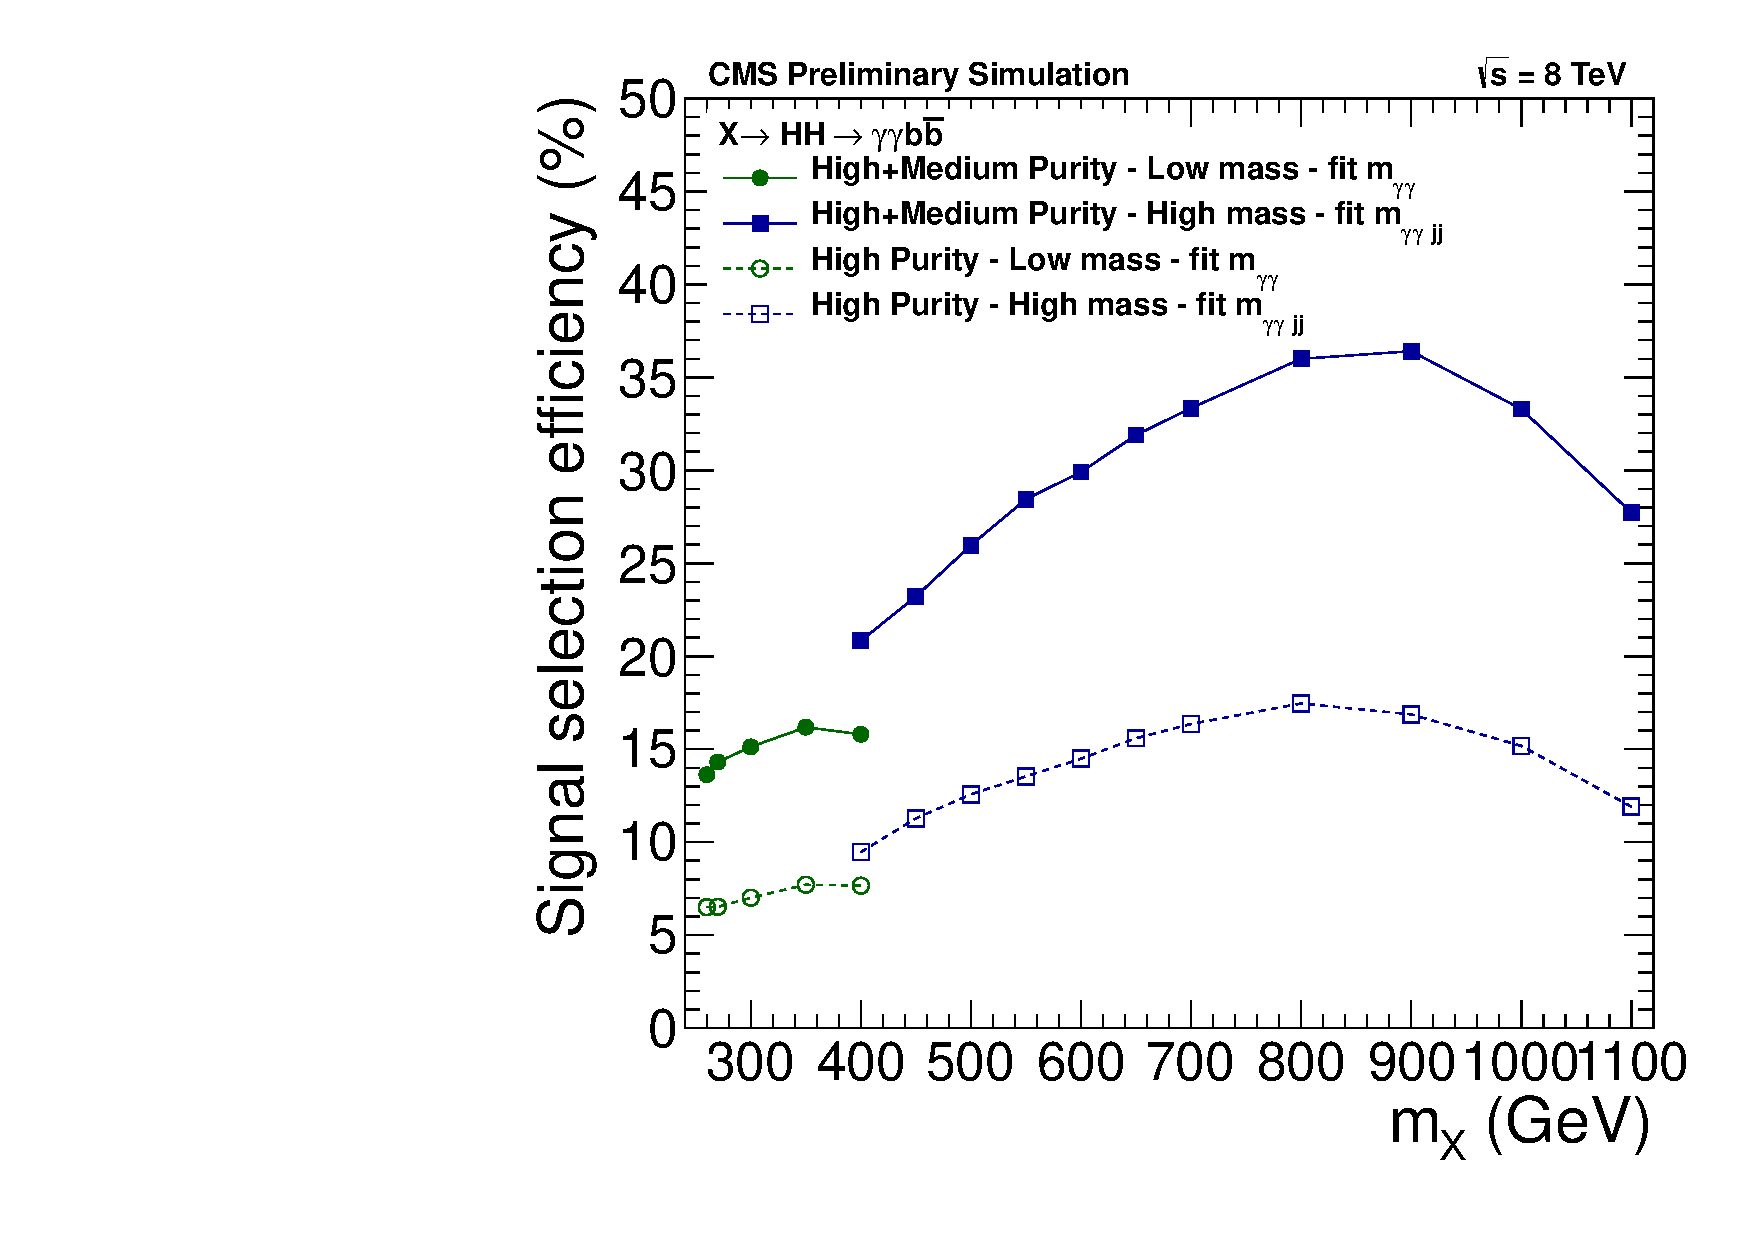
\includegraphics[width=0.70\textwidth]{figures/results/eff_all.pdf}
      \end{center}
\caption{Signal efficiency for the resonant search for final selection.}
\label{fig:eff_res}
\end{figure}

The yields for the low-mass resonant search at $m_X = 300$~GeV are summarized in
Table~\ref{table:yield_lowmass_res}. Note that there is a normalization disagreement in the
$\gamma\gamma j$ and $\gamma j$ contributions as the simulation has limitations in modeling
QCD with one or two hard photons. As a result, the backgrounds are not added; the purpose is to
highlight relative contributions. The yields for the high-mass resonant search are summarized in
Table~\ref{table:yield_highmass_res}. For this search, the requirements are independent of
the mass hypothesis, so a several signal hypotheses can be shown together.

\begin{table}[ht]
  \centering
  \renewcommand{\arraystretch}{1.4}
  \caption{Event yields for the low-mass resonant search at 300 GeV. Expectations are given for
the signal, resonant background, and nonresonant background. Counts are given for data. Note that
there is a normalization disagreement coming from the shortcomings of simulating QCD with one
or two hard photons.}
  \begin{tabular}{|c|c|c|}
\hline
Sample & High purity & Medium purity\\
\hline
Radion (300$~$GeV, $\Lambda_R$=1TeV)  & 18.73 & 21.66     \\
\hline
ggF $\Hgg$                &  0.02  &  0.19 \\
VBF $\Hgg$                &  0.00  &  0.04 \\
$WH(\gamma\gamma)$        &  0.00  &  0.05 \\
$ZH(\gamma\gamma)$        &  0.00  &  0.03 \\
$t\bar{t}H(\gamma\gamma)$ &  0.10  &  0.15 \\
\hline
$\gamma\gamma j$                      & 8.9  &  188  \\
$\gamma j$                            & 0.00 &  9.2  \\ 
QCD                                   & 0.00 &  0.00 \\ 
$Z/\gamma^*\rightarrow\ell^+\ell^- + Z(\ell^+\ell^-)\gamma + W(\ell\nu)\gamma\gamma$ & 0.00 &  0.21 \\
$t\bar{t}\gamma\gamma + t\gamma\gamma + t\bar{t}\gamma j$ & 0.44 &  1.2  \\
\hline
Data                                  & 21 & 230 \\
\hline
\end{tabular}

  \label{table:yield_lowmass_res}
\end{table}

\begin{table}[ht]
  \centering
  \renewcommand{\arraystretch}{1.4}
  \caption{Event yields for the high-mass resonant search. Expectations are given for
the signal, resonant background, and nonresonant background. Counts are given for data. Note that
there is a normalization disagreement coming from the shortcomings of simulating QCD with one
or two hard photons.}
  \begin{tabular}{|c|c|c|}
\hline
Sample & High purity & Medium purity\\
\hline
Radion (500$~$GeV, $\Lambda_R$=1TeV)        &  6.08  & 6.47     \\
Radion (700$~$GeV, $\Lambda_R$=1TeV)        &  2.92  & 3.03     \\
Radion (1000$~$GeV, $\Lambda_R$=1TeV)       &  0.94  & 1.12     \\
\hline
ggF $\Hgg$                &  0.07  &  0.6  \\
VBF $\Hgg$                &  0.01  &  0.12 \\
$WH(\gamma\gamma)$        &  0.00  &  0.10 \\
$ZH(\gamma\gamma)$        &  0.03  &  0.07 \\
$t\bar{t}H(\gamma\gamma)$ &  0.24  &  0.50 \\
\hline
$\gamma\gamma j$                      & 3.0  &  70   \\
$\gamma j$                            & 0.00 &  3.0  \\
QCD                                   & 0.00 &  0.00 \\
& 8.9  &  188  \\
& 0.00 &  9.2  \\ 
& 0.00 &  0.00 \\ 
$Z/\gamma^*\rightarrow\ell^+\ell^- + Z(\ell^+\ell^-)\gamma + W(\ell\nu)\gamma\gamma$ & 0.00 &  0.08 \\
$t\bar{t}\gamma\gamma + t\gamma\gamma + t\bar{t}\gamma j$ & 0.15 &  0.55 \\
\hline
Data                                  & 8 & 79 \\
\hline
\end{tabular}

  \label{table:yield_highmass_res}
\end{table}

The yields for the nonresonant search are summarized in Table~\ref{table:yield_nonres}.
The yields are higher in the nonresonant search because the $\Mggjjk$ spectrum is much less
disciminating than in the low-mass resonant search and because the $\Mjj$ is fit rather than
selected.

\begin{table}[ht]
  \centering
  \renewcommand{\arraystretch}{1.4}
  \caption{Event yields for the nonresonant search. Expectations are given for
the SM nonresonant signal, resonant background, and nonresonant background.
Counts are given for data. Note that
there is a normalization disagreement coming from the shortcomings of simulating QCD with one
or two hard photons.}
  \begin{tabular}{|c|c|c|c|c|}
\hline
 & \multicolumn{2}{c|}{High Purity} & \multicolumn{2}{c|}{Medium Purity} \\
Sample & high $\Mggjjk$ & low $\Mggjjk$ & high $\Mggjjk$ & low $\Mggjjk$ \\
\hline
SM nonresonant $HH$ & 2.03 & 0.28 & 1.99 & 0.20\\
%SM: $\kapl = 1$, $\kapt = 1$, $\ctwo = 0$ & 2.03 & 0.28 & 1.99 & 0.20\\
%$\kapl = 20$, $\kapt = 1$, $\ctwo = 0$ & 78.7 & 102 & 86.5 & 96.5\\
%$\kapl = 1$, $\kapt = 1$, $\ctwo = -2$  & 103 & 16.2 & 101 & 16.5\\
%lam=1  yt=1 c2=0  xsec = 9.96
%lam=20 yt=1 c2=0  xsec = 1046
%lam=1  yt=1 c2=-2 xsec  = 511
\hline
ggF $\Hgg$                &  0.05 & 0.04 & 0.29 & 0.32\\
VBF $\Hgg$                &  0.01 & 0.01 & 0.05 & 0.05\\
$WH(\gamma\gamma)$        &  0.00 & 0.00 & 0.12 & 0.09\\     
$ZH(\gamma\gamma)$        &  0.04 & 0.02 & 0.07 & 0.05\\
$t\bar{t}H(\gamma\gamma)$ &  0.16 & 0.17 & 0.30 & 0.17\\
$b\bar{b}H(\gamma\gamma)$ &  0.00 & 0.01 & 0.01 & 0.04\\  
\hline
$\gamma\gamma j$     &  13 & 21  & 151 & 268 \\
$\gamma j$           & 0.00& 4.3 & 28  & 53  \\
QCD                  & 0.00& 0.00& 0.00& 0.00\\
$Z/\gamma^*\rightarrow\ell^+\ell^- + Z(\ell^+\ell^-)\gamma + W(\ell\nu)\gamma\gamma$
   & 0.00 & 0.01 & 2.3 & 0.18 \\
$t\bar{t}\gamma\gamma + t\gamma\gamma + t\bar{t}\gamma j$ &  1.3 & 2.2 & 3.3 & 3.4 \\
\hline
Data                                  & 41 & 136 & 37 & 319 \\
\hline
\end{tabular}

  \label{table:yield_nonres}
\end{table}

\section{Resonant Results\label{sec:resresults}}

\subsection{Low-mass Resonant Results}

For the low-mass resonant search, the signal yield is extracted by fitting the $\Mgg$ spectrum.
The signal model is built for each mass hypthesis by fitting the $\Mgg$ peak in the simulation
separately for the two categories. This functional form used is the sum of a Crystal Ball and
Gaussian, where the former models the core of the distribution and the latter models the
tails. The position of the peak and the spread having no dependence on the resonant mass and the
category. Figure~\ref{fig:sigfit_300} shows an example of the signal fit for a signal of mass 300 GeV.

\begin{figure}[ht]
 \begin{center}
   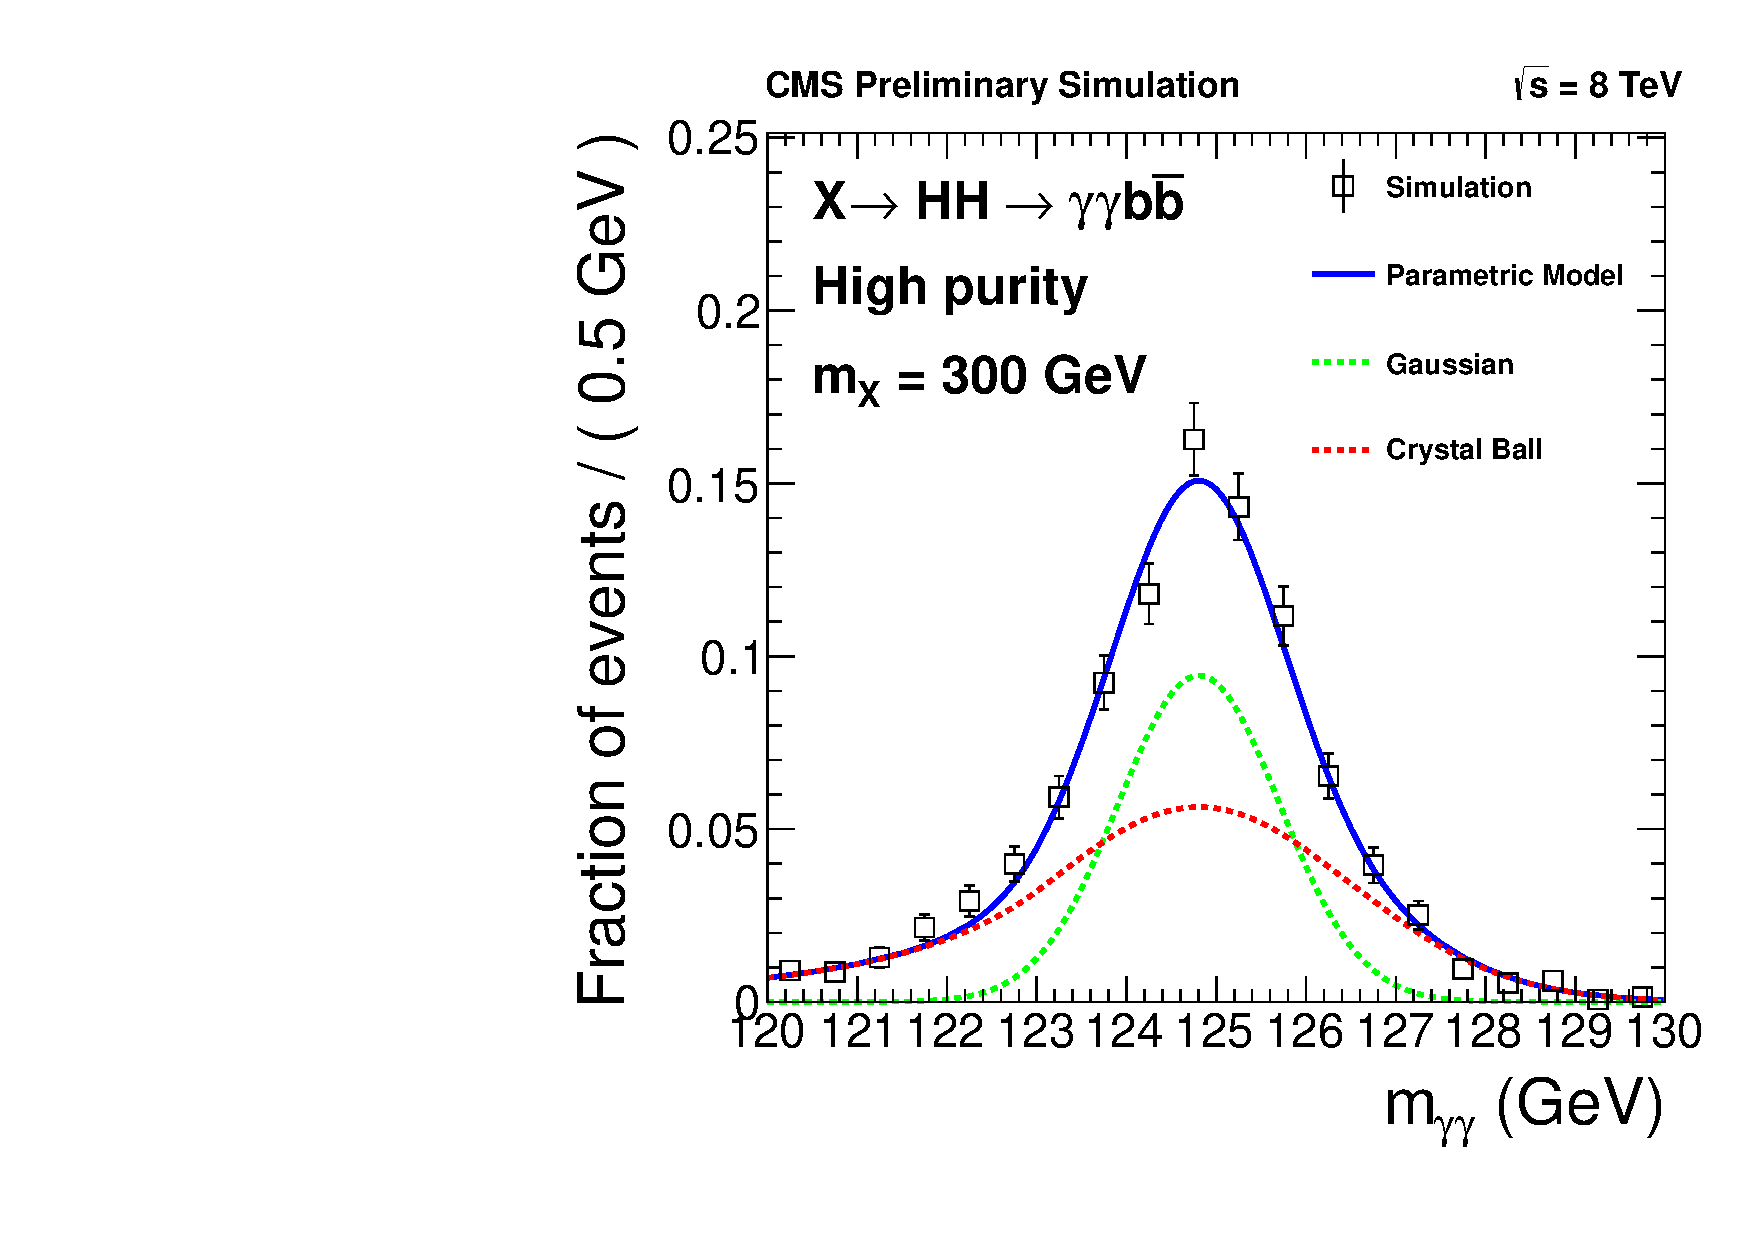
\includegraphics[width=0.70\textwidth]{figures/results/sigmodel_cat0_300.pdf}
   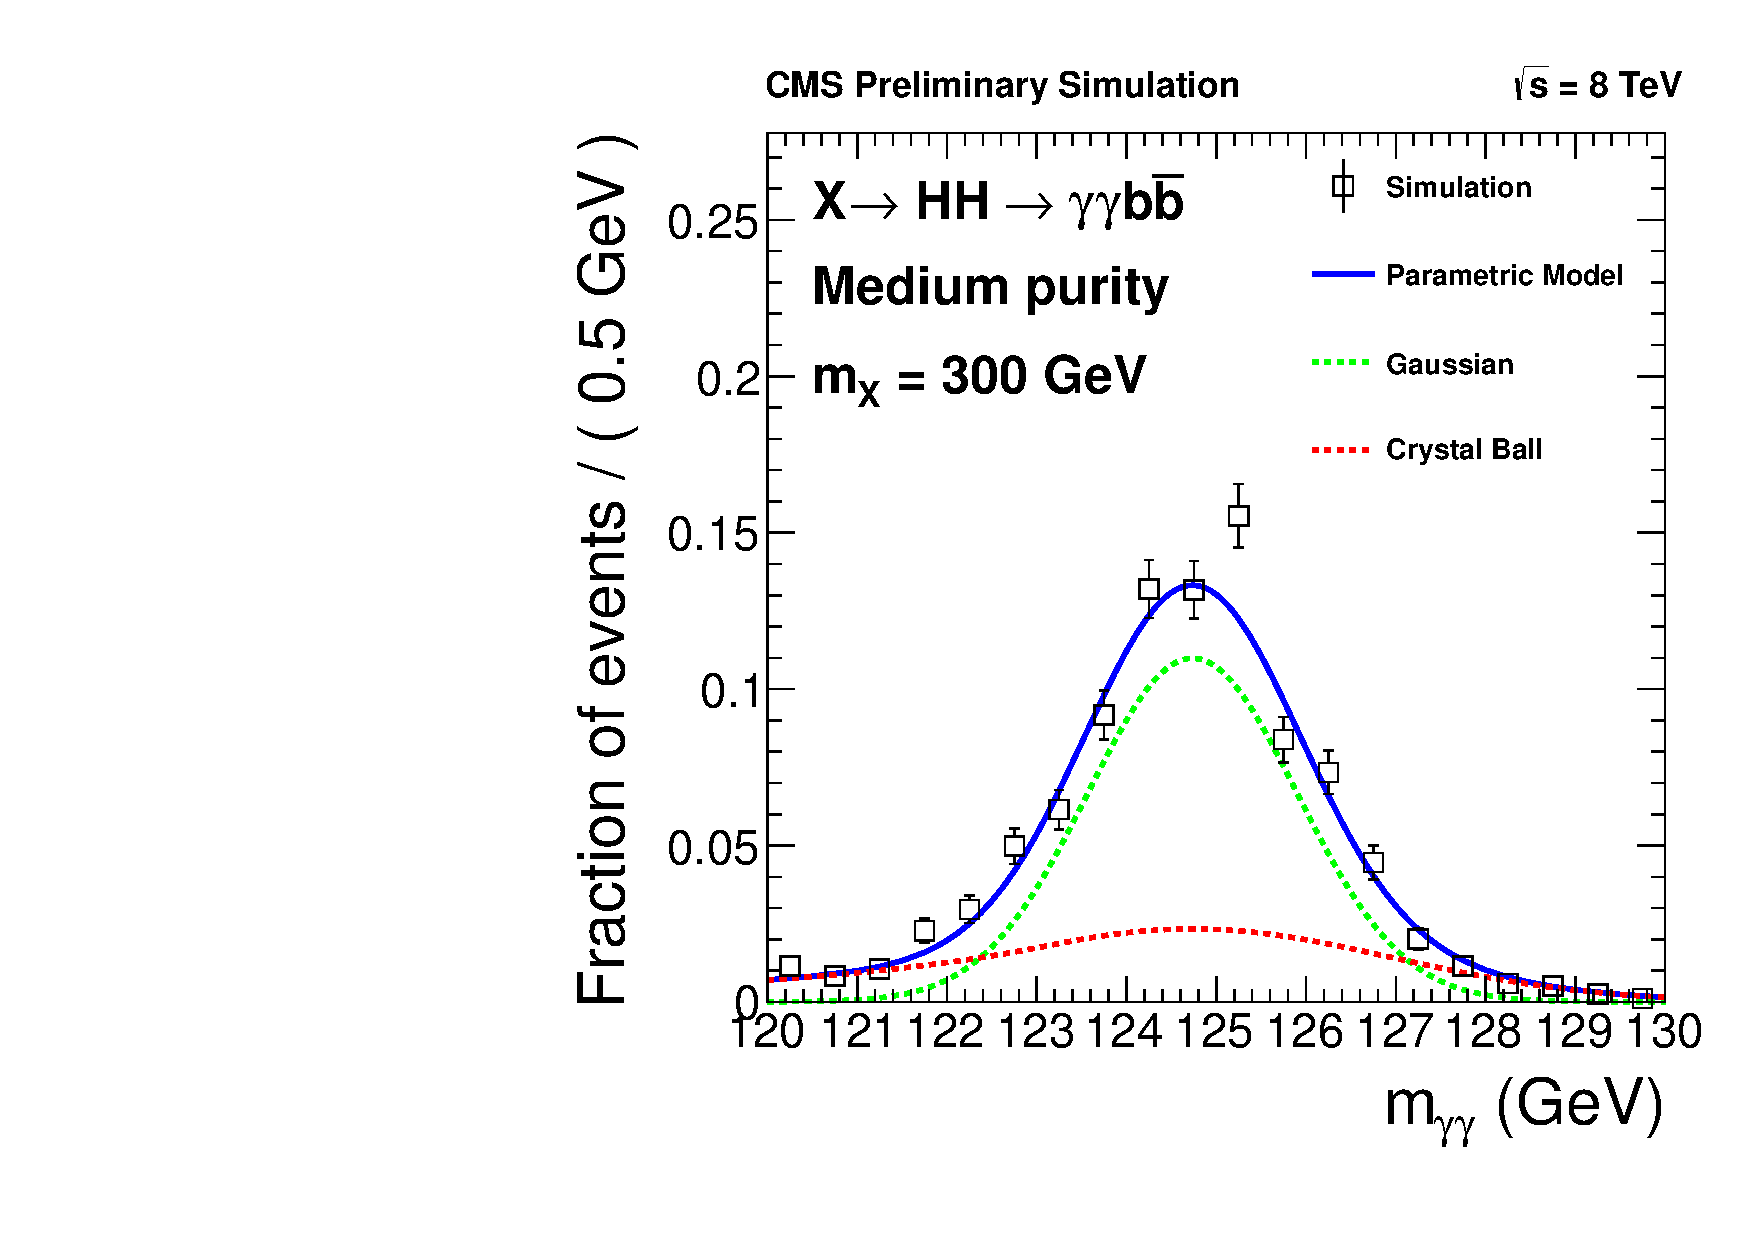
\includegraphics[width=0.70\textwidth]{figures/results/sigmodel_cat1_300.pdf}
 \end{center}
\caption{Simulated signal shape in the $\Mgg$ spectrum for the high-purity (top) and medium-purity
(bottom) categories for the Radion with mass 300 GeV. The open squares and corresponding
statistical uncertainties represent the simulation.
The blue line represents the model fitted to the simulation, while the green dashed line
and the red dashed line represent the two components of the model.}
\label{fig:sigfit_300}
\end{figure}

The background estimation is done by fitting the same distribution in each category on the interval
$[100, 180]$~GeV. This procedure is completely data-driven procedure, and as such it is important
that the choice of the function does not bias in a non-negligible way the estimate of the signal
strength obtained from the model conbining signal and background components.
The bias is estimated by considering a set of truth models which approximately describe the background.
For each truth model a large set of pseudo-data is generated and fitted by the sum of a candidate
background model and the signal model. The bias is defined as the ratio of the extracted signal strength
$\mu$ divided by the associated statistical uncertainty $\sigma_\mu$.
The bias is considered negligible if
\begin{equation}
\left|\text{median}\left(\frac{\mu}{\sigma_\mu}\right)\right| < 14\% \,.
\end{equation}
For both categories, more than one unbiased function was identified. For the limit extraction,
a power law is used for both categories. Figure~\ref{fig:datafit_300} shows these fits to the
data for four mass hypotheses.

\begin{figure}[ht]
 \begin{center}
   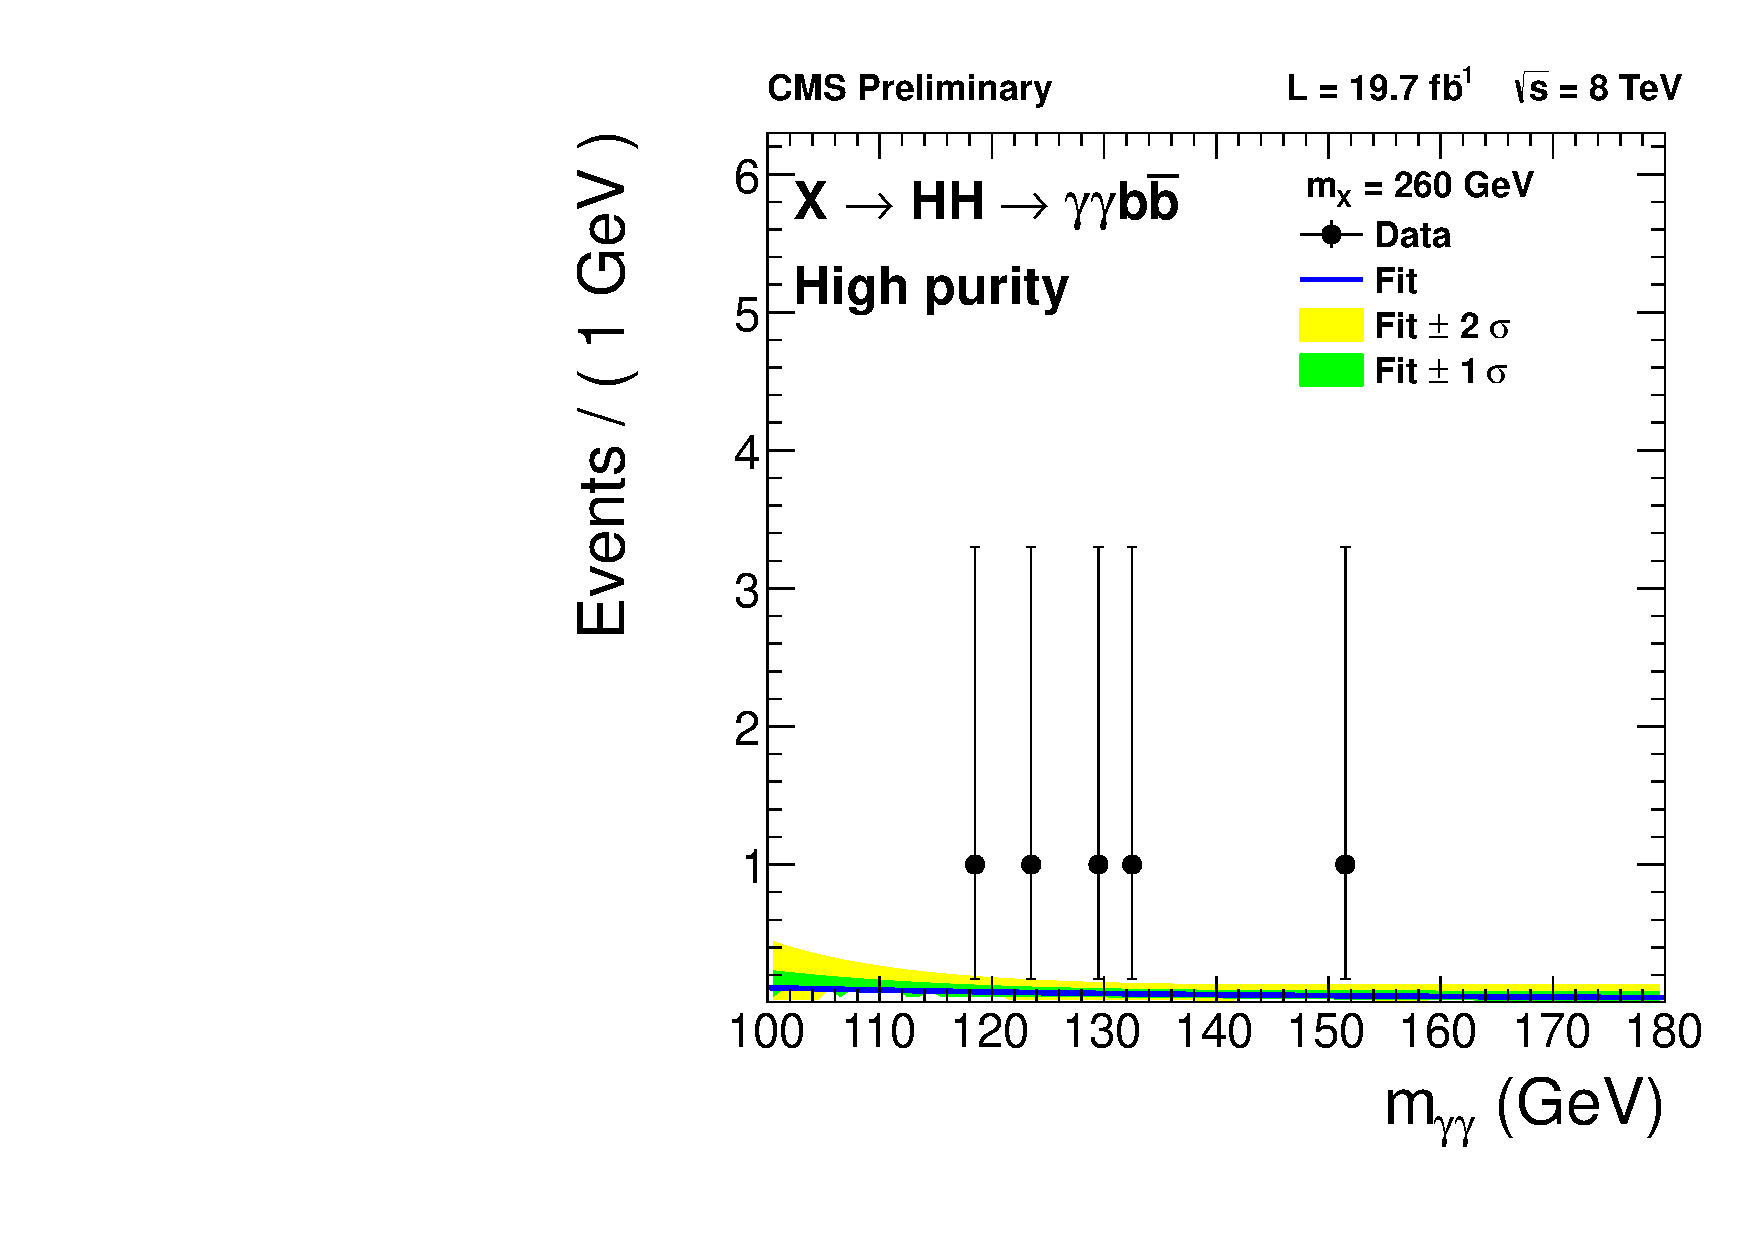
\includegraphics[width=0.45\textwidth]{figures/results/databkgoversig_cat0_260GeV.pdf}
   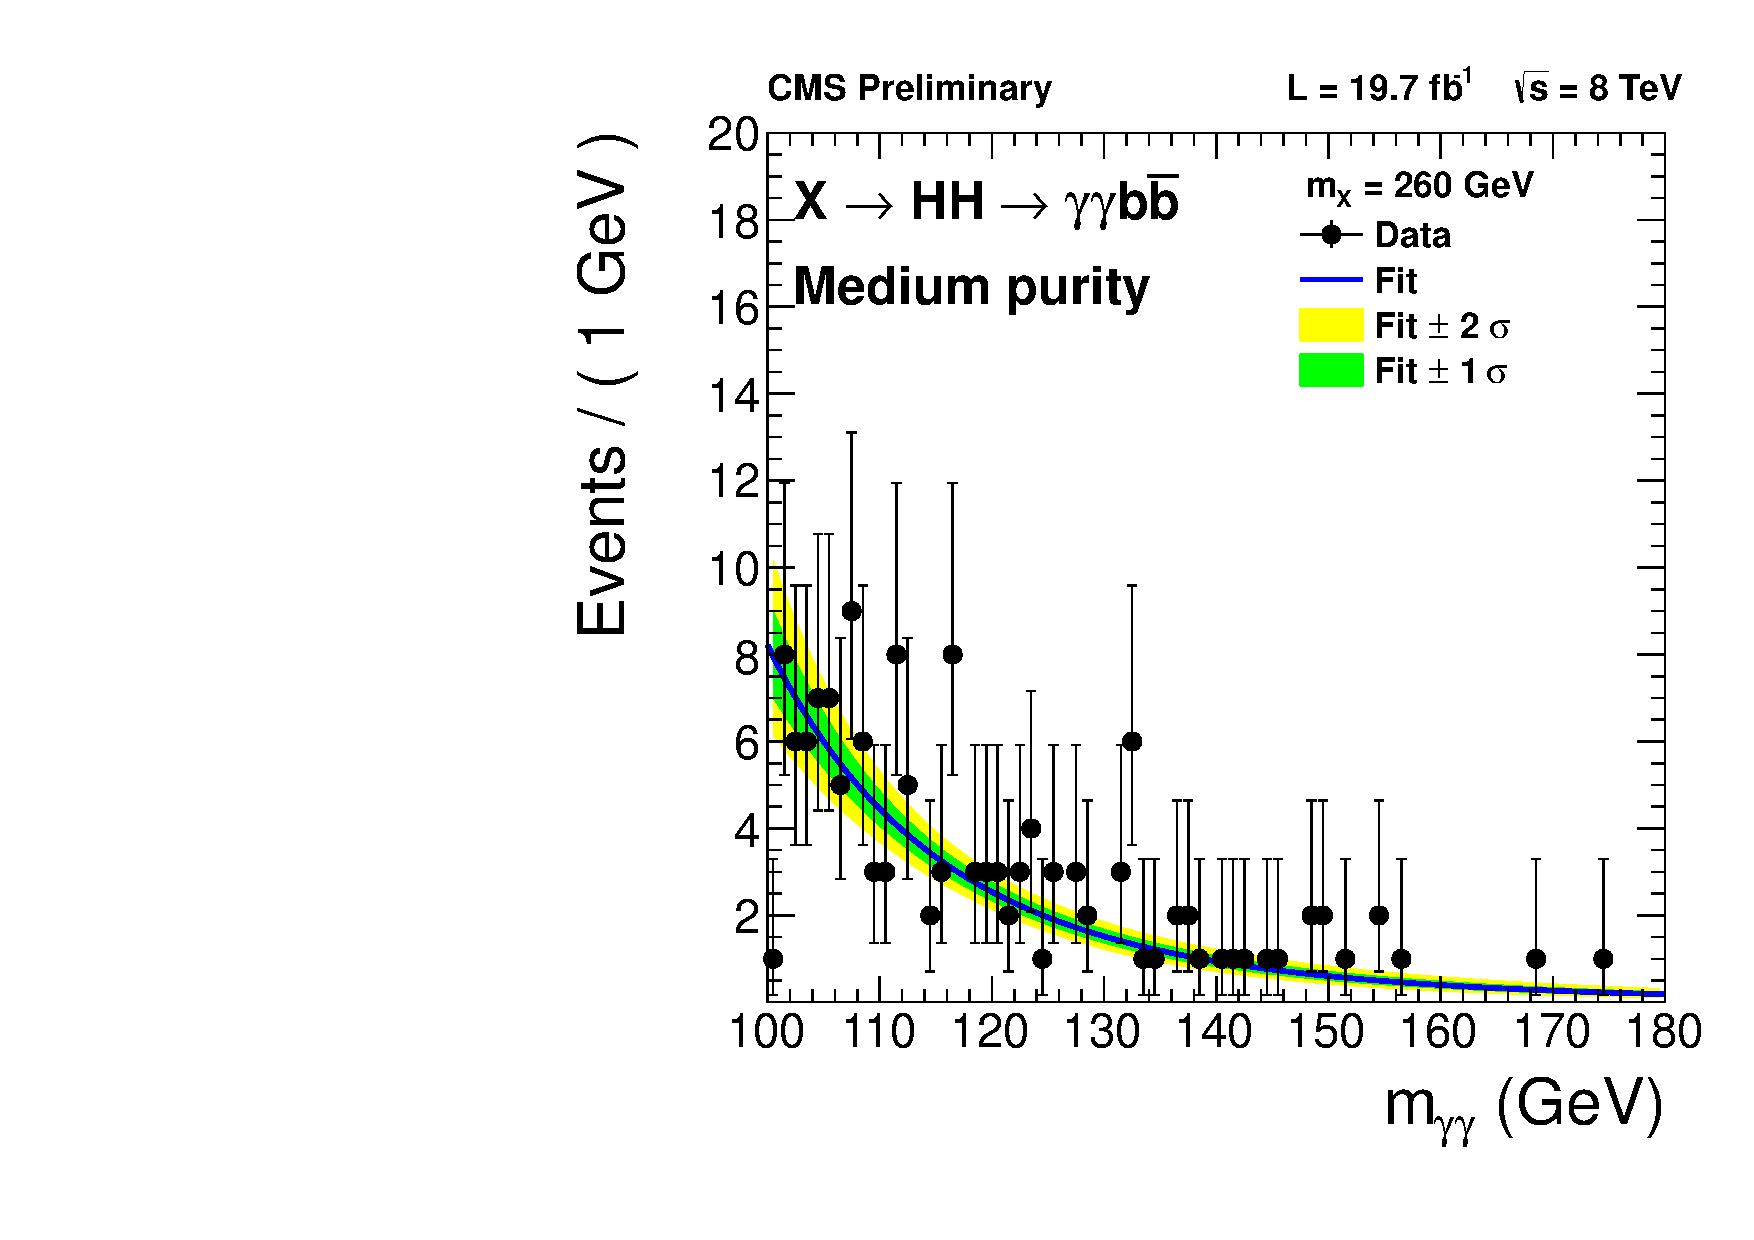
\includegraphics[width=0.45\textwidth]{figures/results/databkgoversig_cat1_260GeV.pdf}
   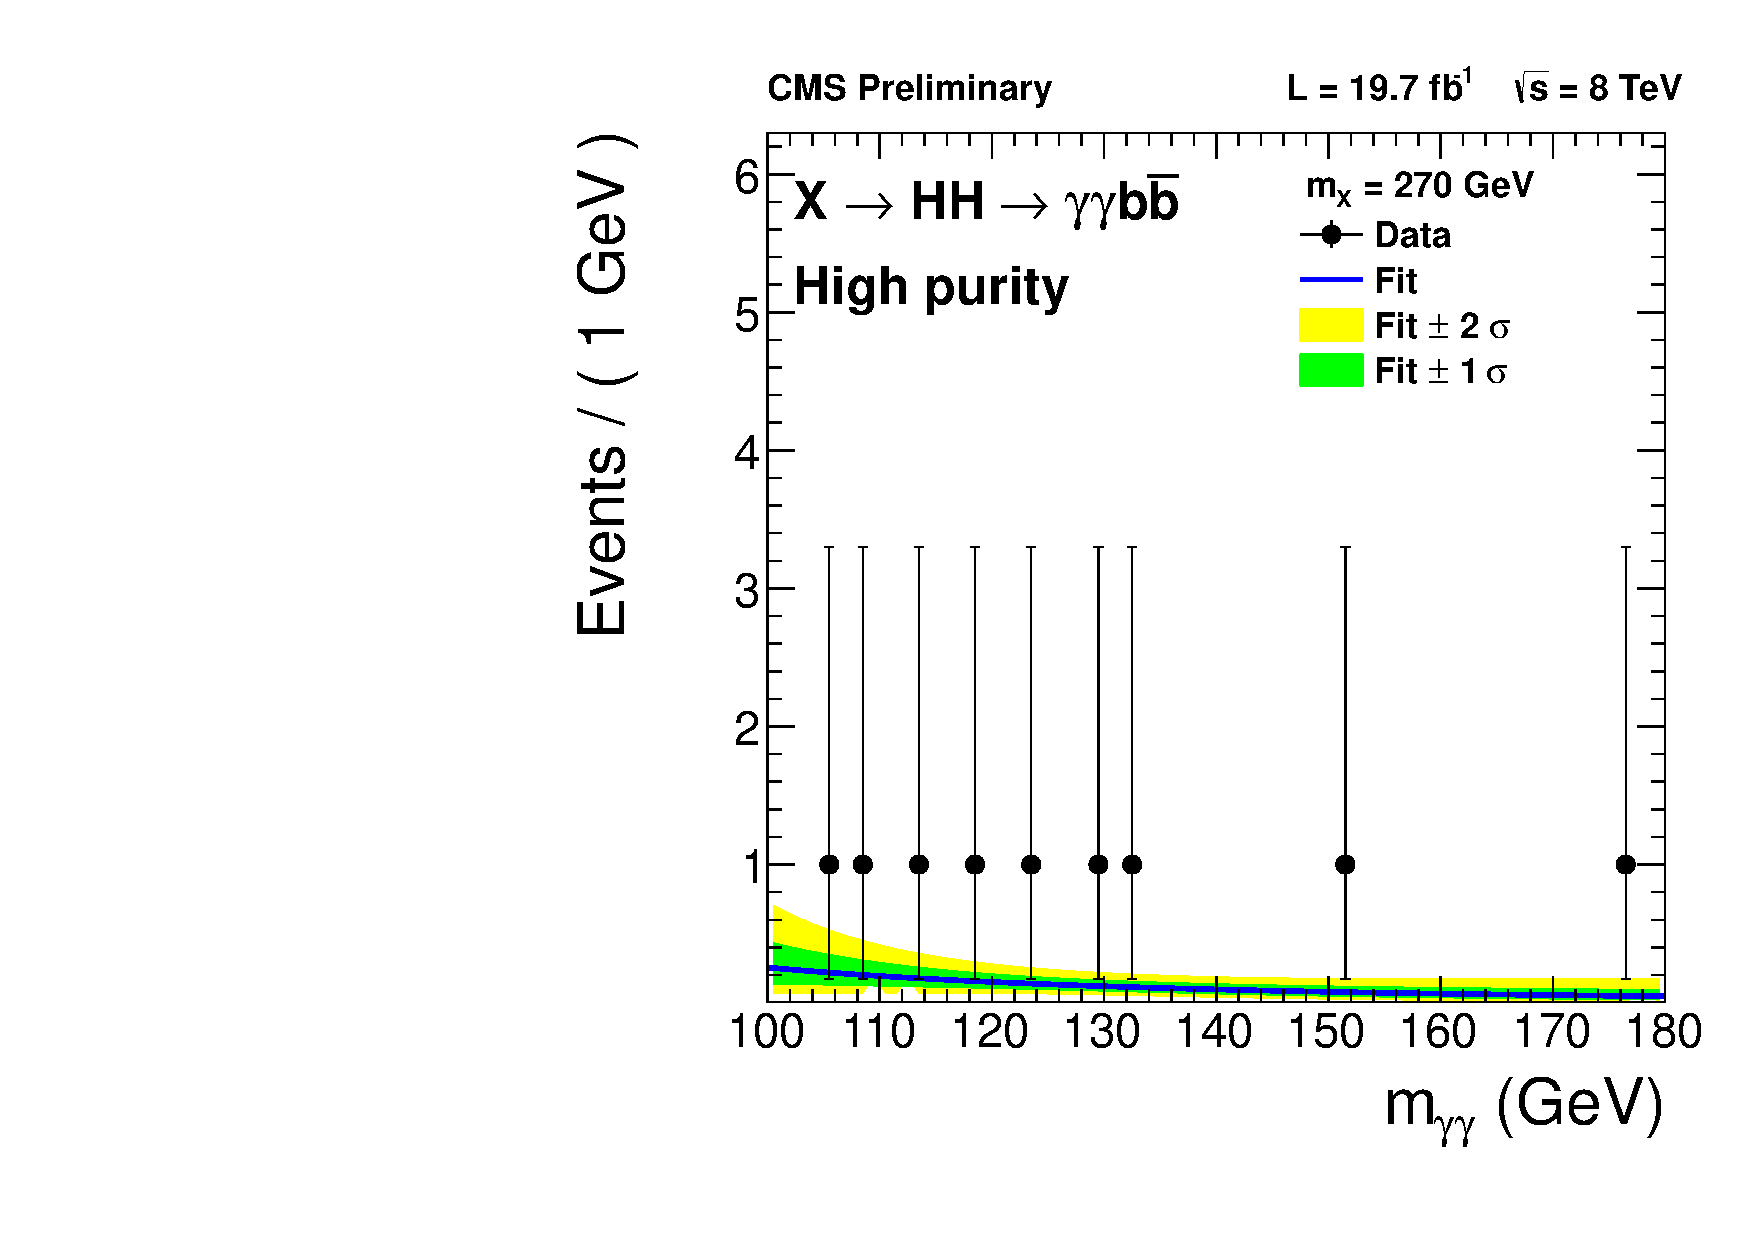
\includegraphics[width=0.45\textwidth]{figures/results/databkgoversig_cat0_270GeV.pdf}
   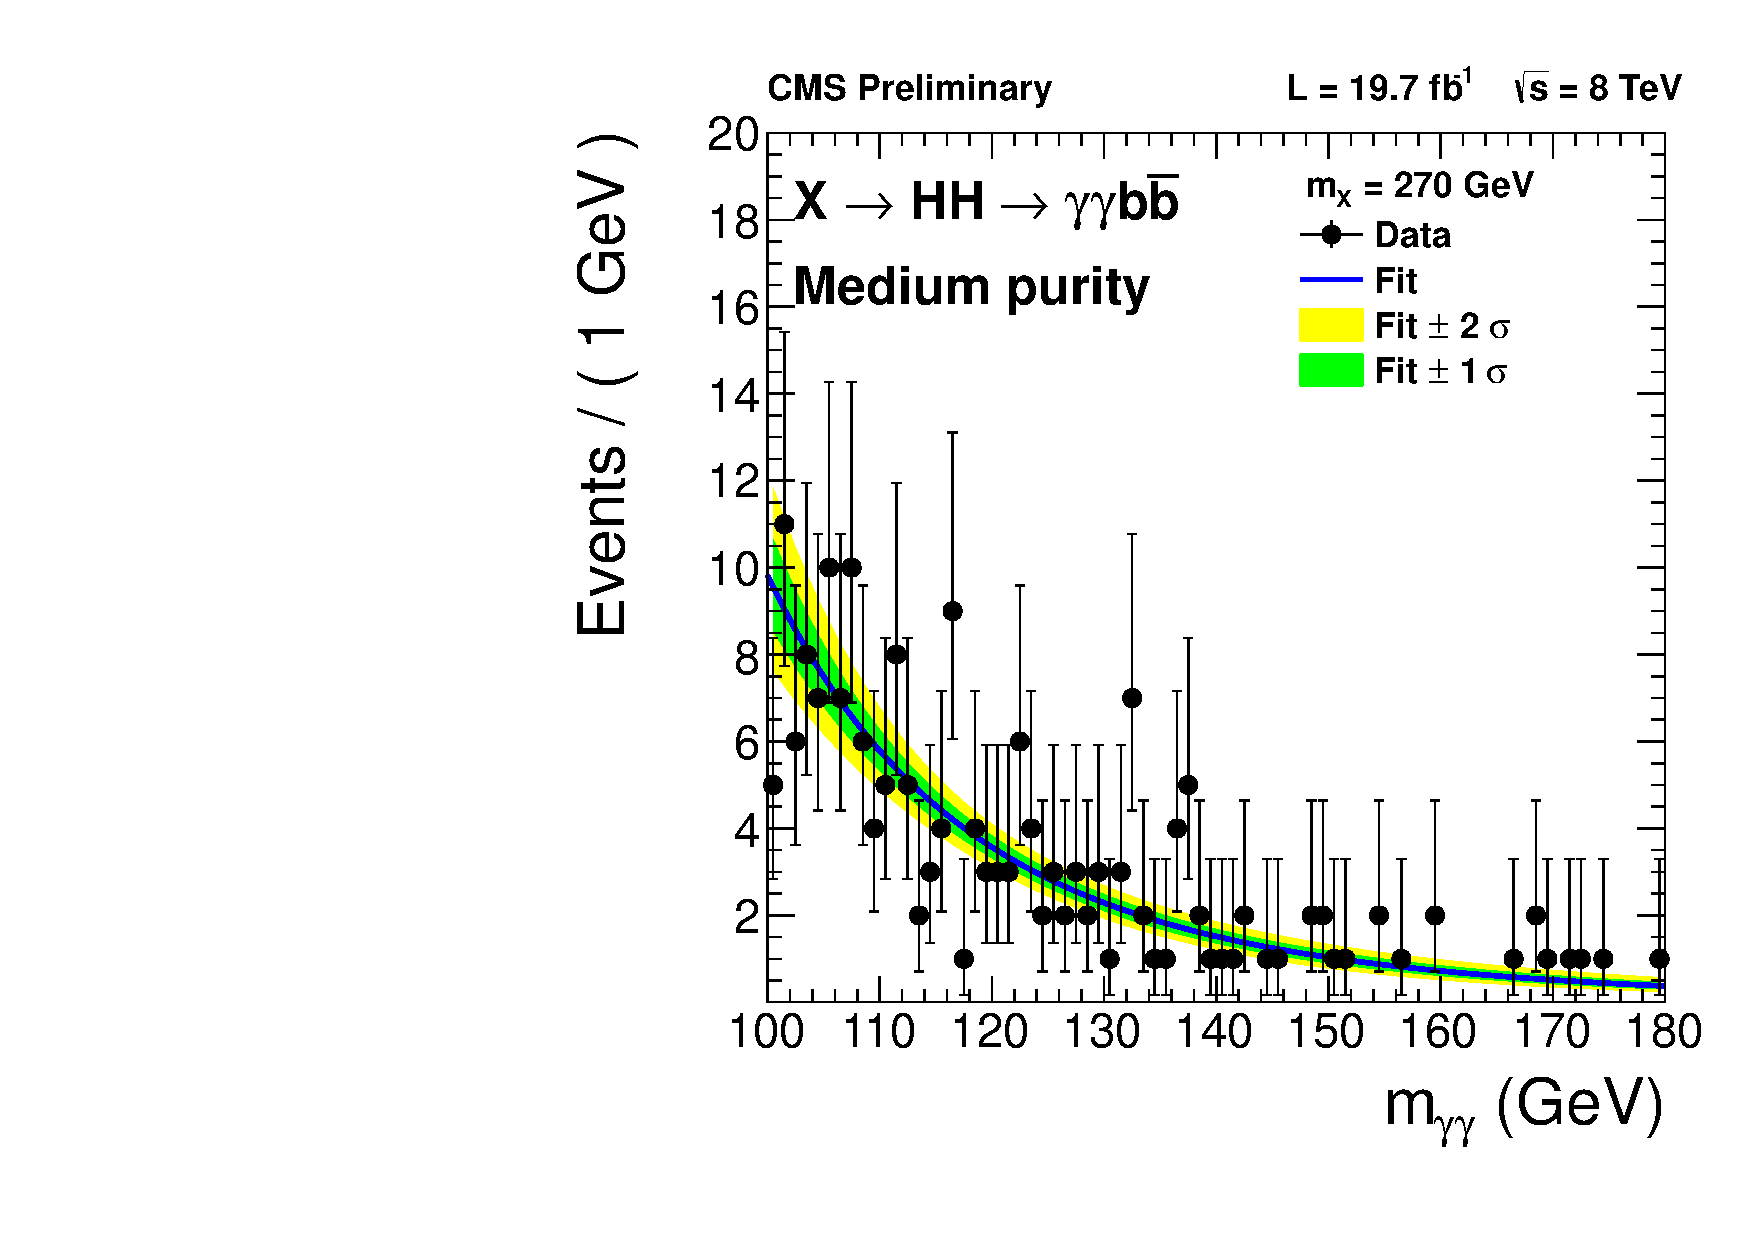
\includegraphics[width=0.45\textwidth]{figures/results/databkgoversig_cat1_270GeV.pdf}
   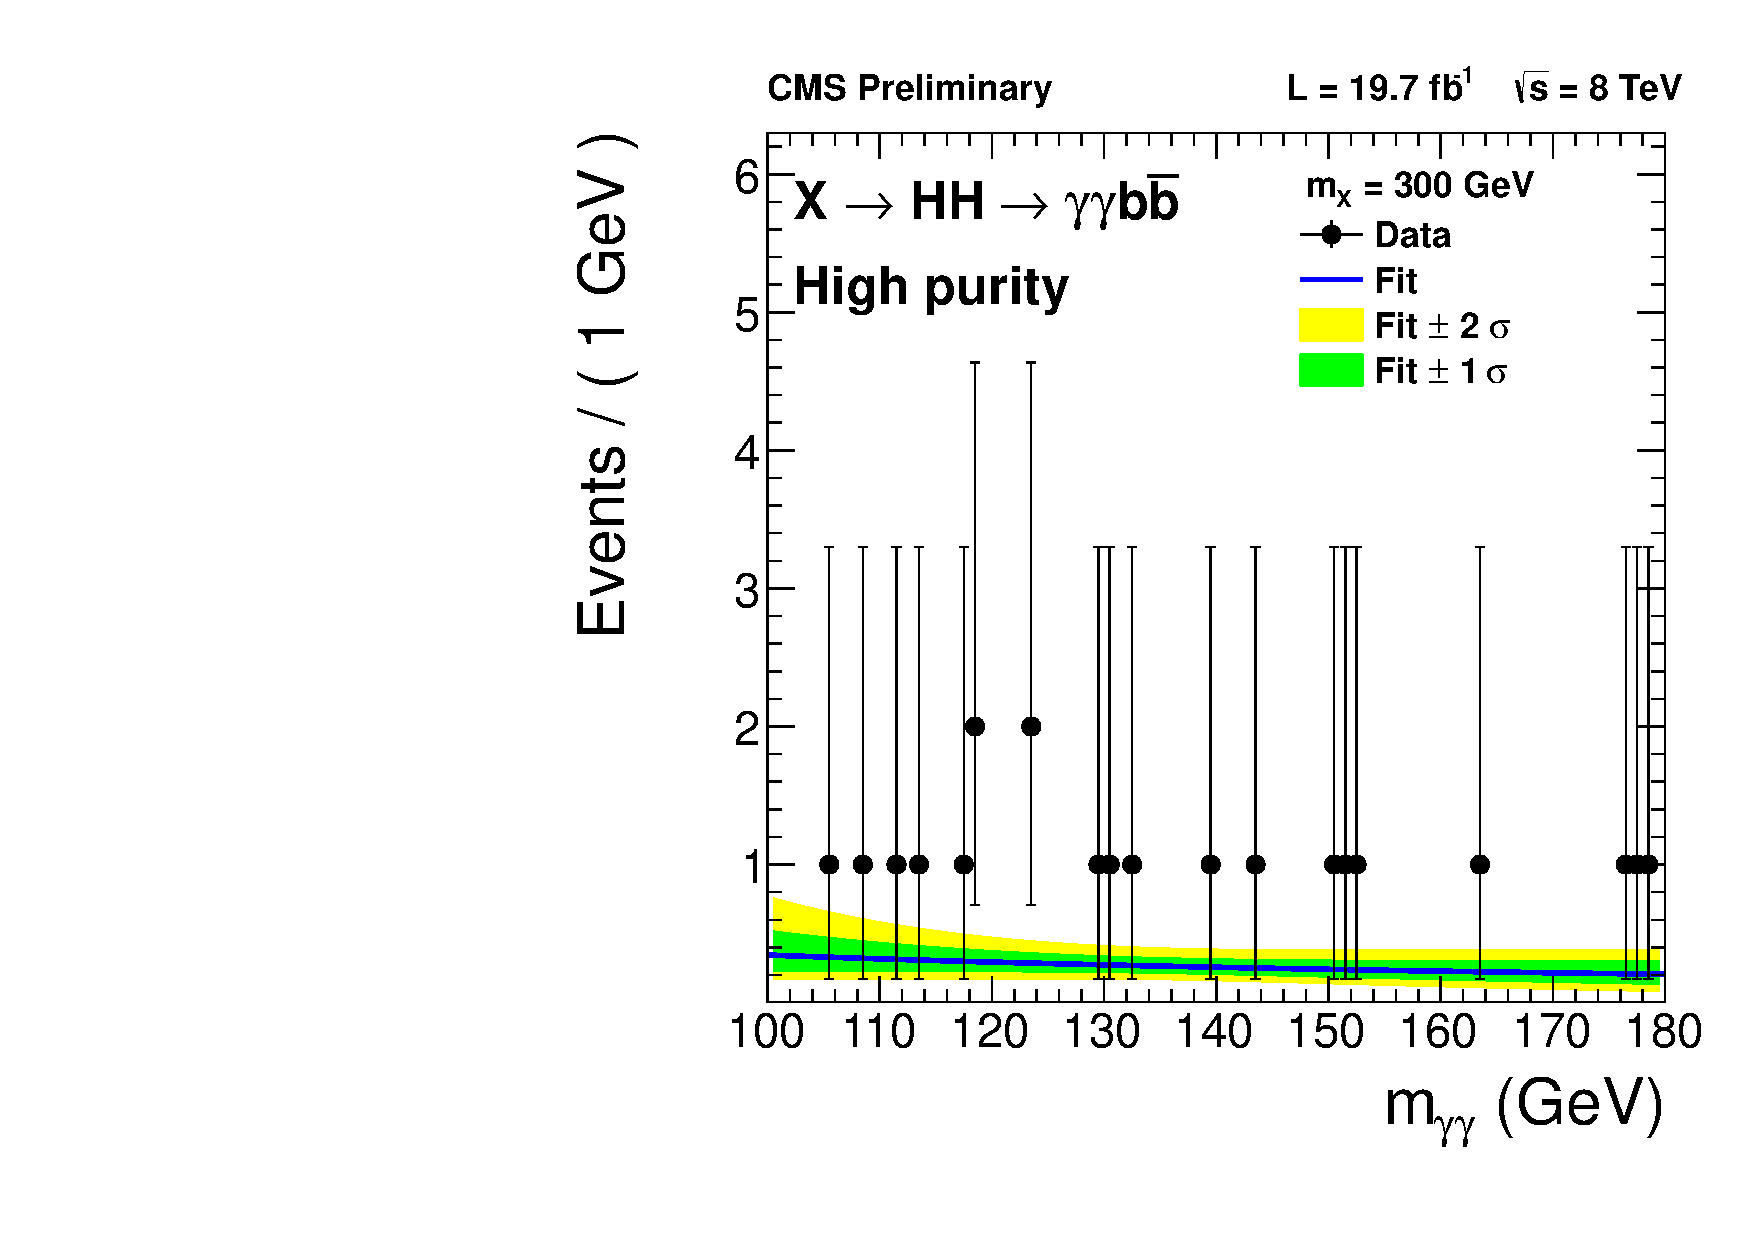
\includegraphics[width=0.45\textwidth]{figures/results/databkgoversig_cat0_300GeV.pdf}
   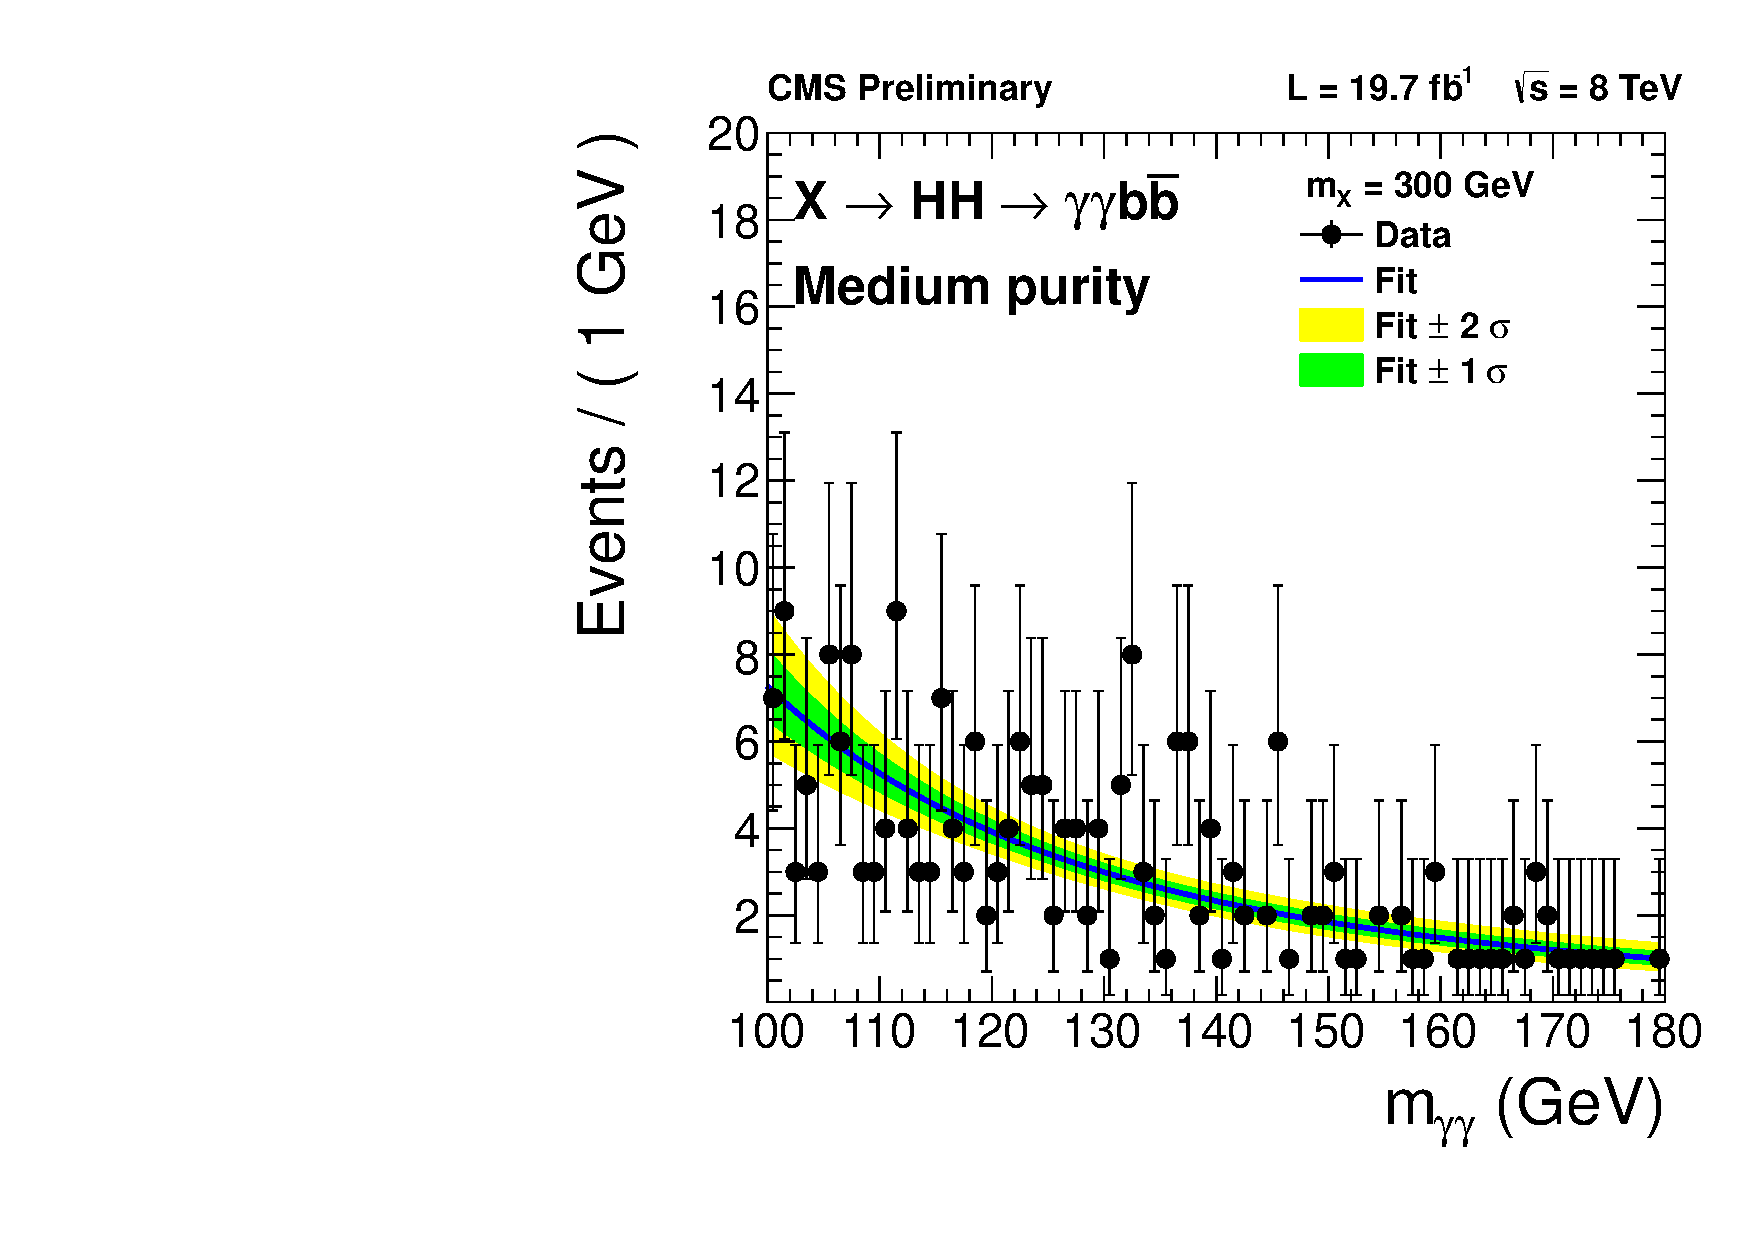
\includegraphics[width=0.45\textwidth]{figures/results/databkgoversig_cat1_300GeV.pdf}
   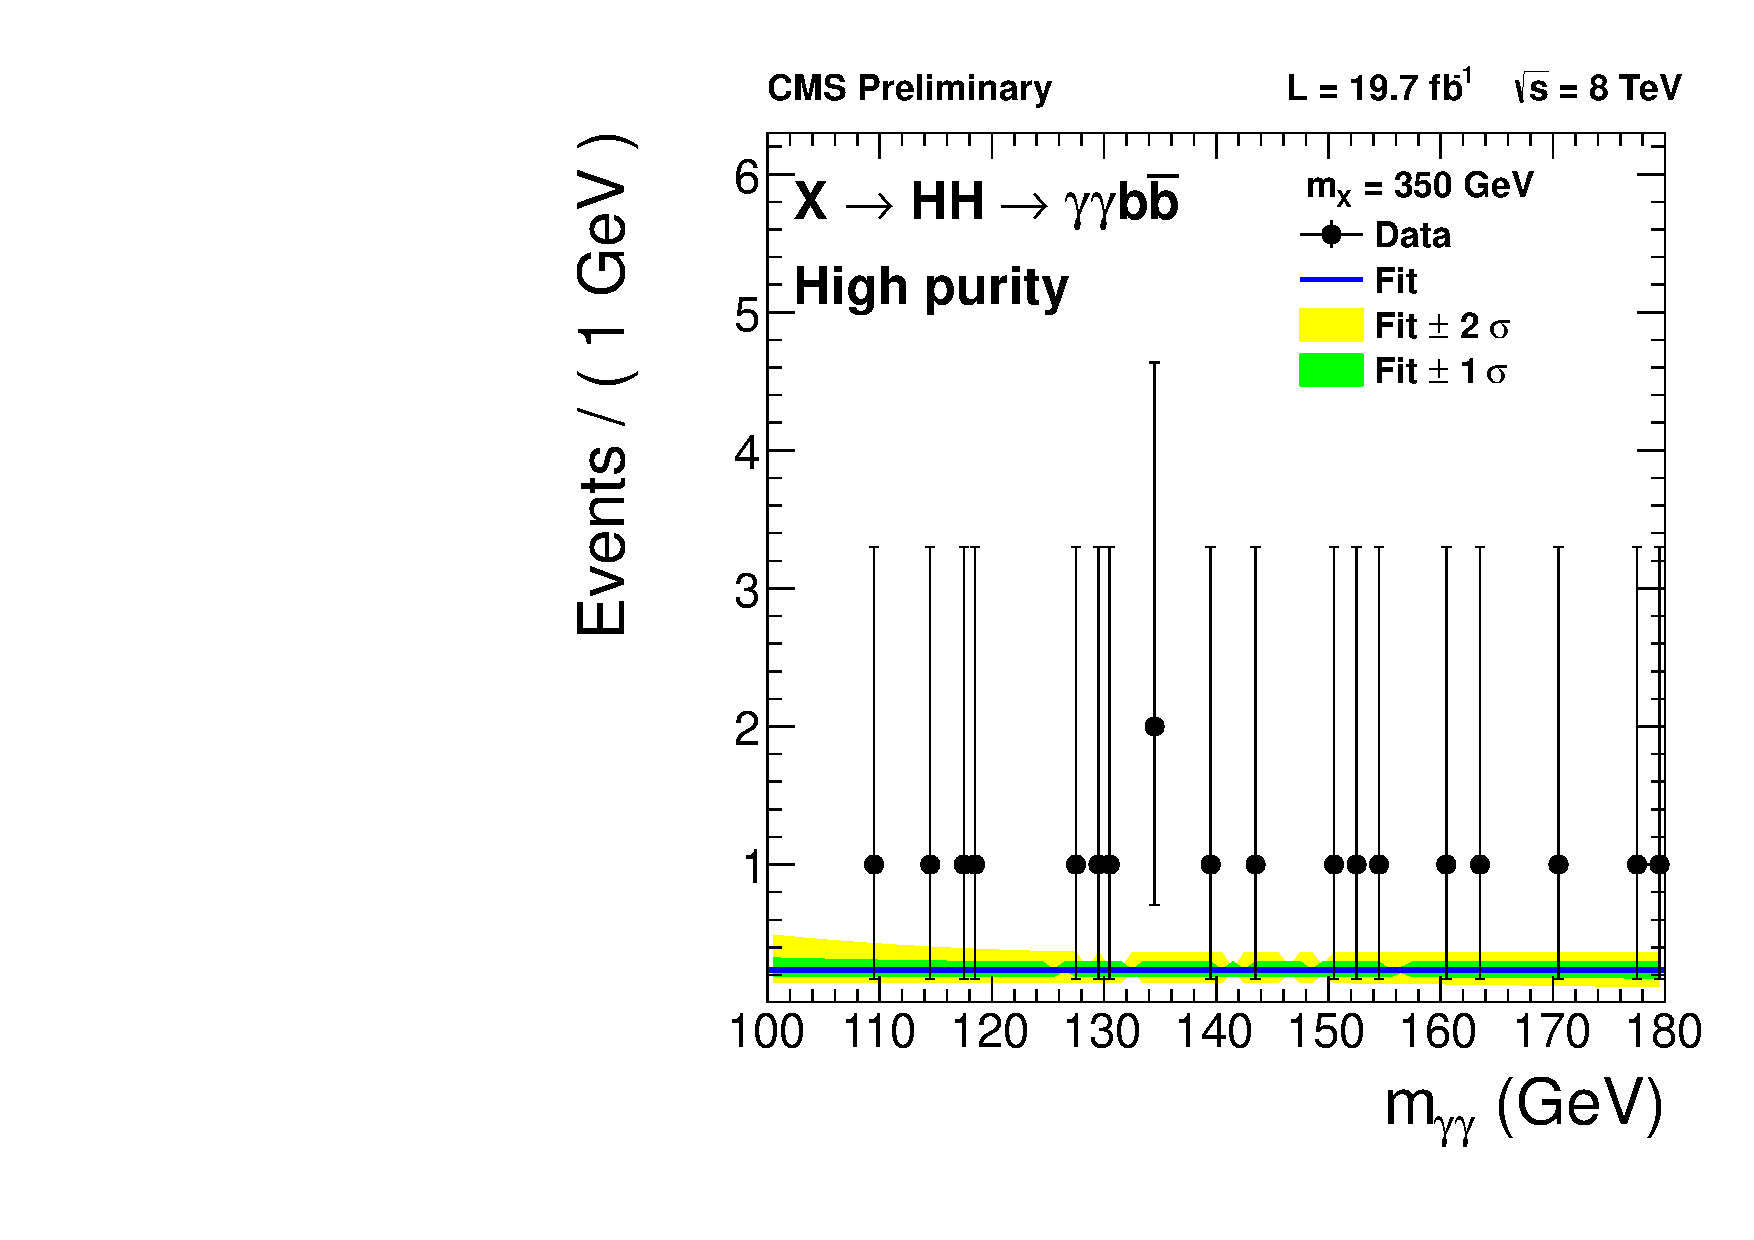
\includegraphics[width=0.45\textwidth]{figures/results/databkgoversig_cat0_350GeV.pdf}
   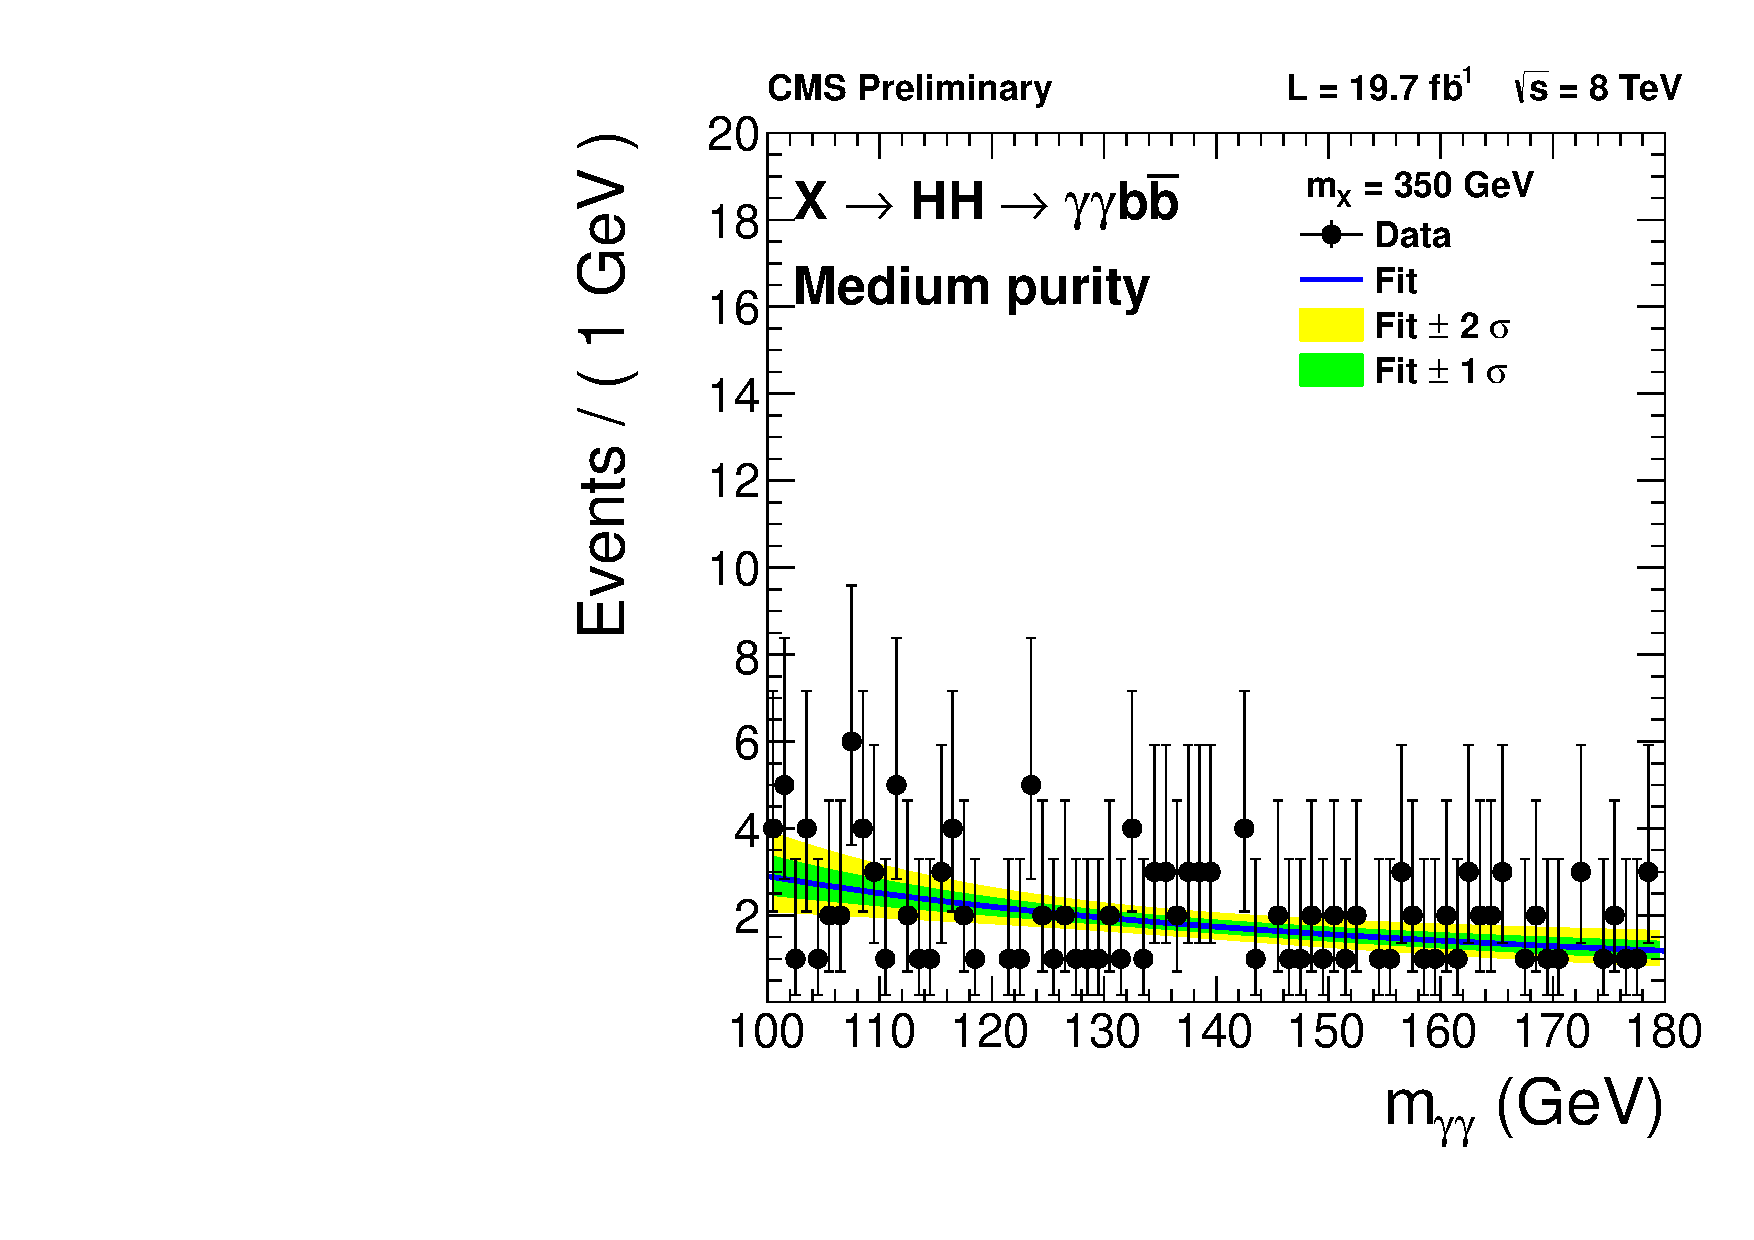
\includegraphics[width=0.45\textwidth]{figures/results/databkgoversig_cat1_350GeV.pdf}
 \end{center}
\caption{Events in the $\Mgg$ spectrum in the high-purity (left column) and medium-purity
(right column) categories for the resonance mass hypotheses 260, 270, 300, and 350 GeV
(from top row down.) The nonresonant component of the background is shown in black
with 1$\sigma$ and 2$\sigma$ bands on the background estimation.}
\label{fig:datafit_300}
\end{figure}

The background fit estimates only the nonresonant contribution arising from diphoton
production. The contribution from SM Higgs production with $\Hgg$ could create a peak in the
spectrum that mimics the signal process. This resonant background
contribution is therefore added in the fit and accounted for in the limits.
The expected contribution of the resonant background is small, and the
effect on the final result is found to be at most 2\%.

There is no excess above the expectation observed, so the analysis proceeds to calculating
upper limits on the signal cross section.
The 95\% CL for expected and observed median upper limits are shown in
Figure~\ref{fig:limits_lowmassres} for both categories and for the high-purity category only.
The latter result is provided to simplify the comparison with new physics models where
the Higgs branching ratios for the $\Hgg$ and $\Hbb$ decays can be modified from the SM.
The green and yellow bands represent the 1$\sigma$ and 2$\sigma$
confidence intervals around the expected limit. Theory expectations for Radion, RS1 KK-graviton, and 
bulk KK-graviton are shown, where the Radion expectation assumes $\text{BR}(R\rightarrow HH) =$~25\%
for all Radion masses above 300 GeV.

\begin{figure}[ht]
 \begin{center}
   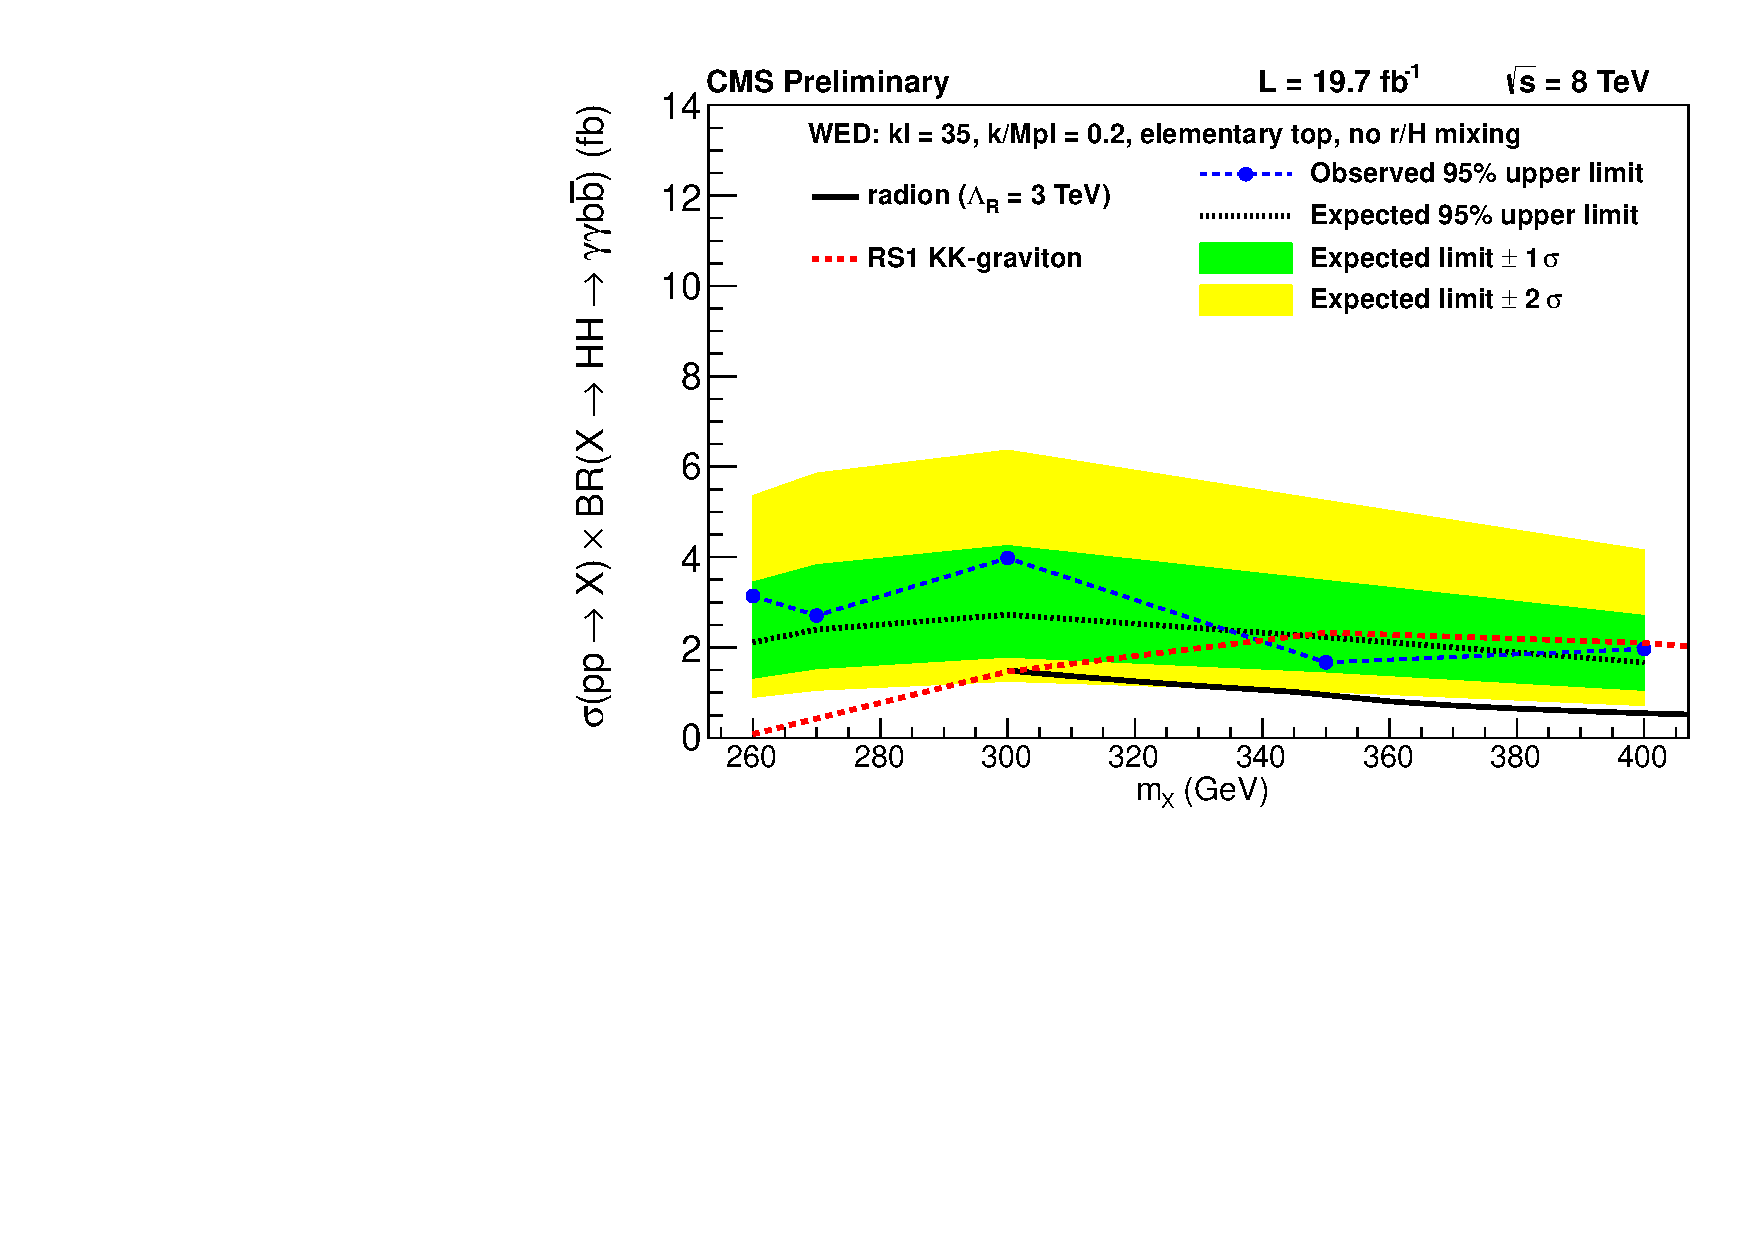
\includegraphics[width=0.7\textwidth]{figures/results/WP4_cutbased_low_all.pdf}
   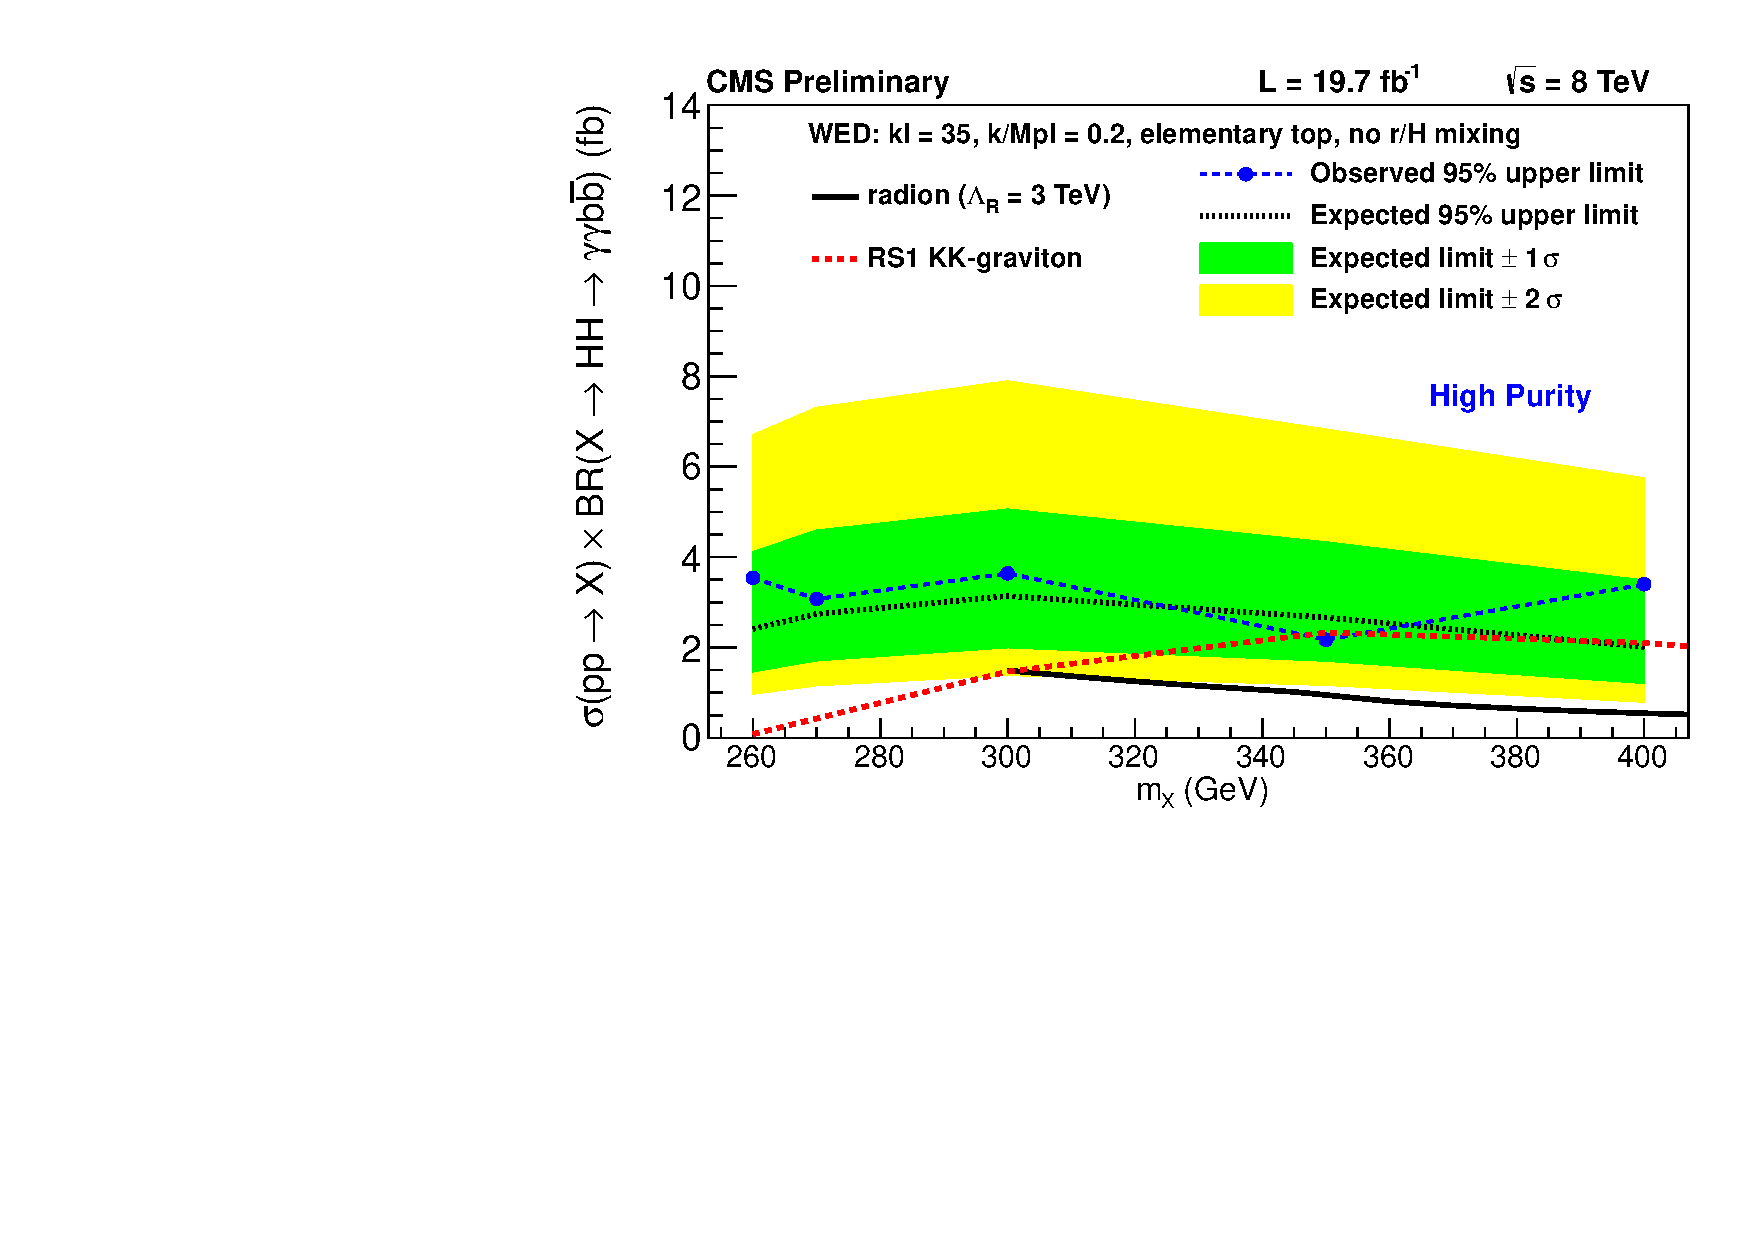
\includegraphics[width=0.7\textwidth]{figures/results/WP4_cutbased_low_base_onecat.pdf}
 \end{center}
\caption{Expected 95\% CL upper limits on the cross section times branching ratios
$\sigma(pp\rightarrow X) \times \text{BR}( X \rightarrow HH \rightarrow \gamma\gamma b\bar{b})$.
Theory lines corresponding to WED models with Radion, RS1 KK-graviton, and bulk KK-graviton are
overlaid. Expected limits from both categories (top) and high-purity category only (bottom) are shown.
The results are obtained using the asymptotic $\text{CL}_s$ approach.}
\label{fig:limits_lowmassres}
\end{figure}

\subsection{High-mass Resonant Results}

The signal is  extracted from a fit  to the
m
kin
gg
jj
spectrum with a  procedure similar to the  one
for  the  low-mass  region.   On  top  of  the  pre-selection  in  Table  1,  the  requirements  12
0
m
g
g
130 GeV and 9
0
m
j
j
165 GeV are applied, the latter being optimized against
the expected limits.
The signal model is built for each mass hypothesis by fitting the
m
kin
gg
jj
distribution in Monte
Carlo separately for the two categories.  A sum of a Crystal Ball and a Gaussian distribution
is used.  The peak position follows the
m
X
evolution while the peak resolution improves for
higher masses,  corresponding to higher momenta of the jets.  The signal fit examples at 500
GeV and 1 TeV are shown on Figure 5.
The background is obtained fitting the
m
kin
gg
jj
distribution for each category in the region defined
by 32
0
m
kin
gg
j
j
1200 GeV. The lower edge is chosen to avoid the kinematic turn-on while still
ensuring full containment of the signal for mass hypotheses
m
X




400 GeV. The same bias esti-
mation procedure described for the low
m
X
region is applied here and the chosen background
fitting function is a power law as shown on Figure 6


include comparison limit plot

\section{Nonresonant Results\label{sec:nonresresults}}

316 The statistical approach used to estimate the significance of a potential excess over the back317
ground and to set the 95% CL expected and observed median upper limits is identical to the
318 resonant search.
319 For the SM-like search waiting unblinding significant excess is observed over the background.
320 The observed (expected) upper limit on the SM-like HH ! ggbb production is waiting un321
blinding (1.54 fb) and waiting unblinding (0.592 pb) for HH production assuming the SM
322 Higgs branching fraction. Using the SMsignal strengthmodificator we also obtain an observed
323 (expected) limit of waiting unblinding (mHH = 61.4), where the uncertainty on the SM cross
324 section prediction was marginalised over.
325 For the interpretation of the BSM-like search we use the LO cross section for di-Higgs produc326
tion expressed in a semi-analytical form as equation 1 [17].
s(pp ! HH) = ¯s
c22
+ (ak2
t )2 + (b kt kl)2 + A1c2(a kt)2 + A2(a k2
t )(b kt kl) + A3 c2(b kt kl)




%\section{The Future\label{sec:future}}

